\documentclass[conf]{new-aiaa}
%\documentclass[journal]{new-aiaa} for journal papers
\usepackage[utf8]{inputenc}
\usepackage{graphicx}
\usepackage{amsmath}
\usepackage{nicefrac}
\usepackage[version=4]{mhchem}
\usepackage{siunitx}
\usepackage{longtable,tabularx}
\setlength\LTleft{0pt} 
\usepackage[table,xcdraw]{xcolor}

\title{On the Efficiency of Higher-Order Implicit Solvers for Compressible Flow
}

\author{Zaid H. Sabri\footnote{Graduate Research Assistant, Mechanical, Industrial, and Manufacturing Engineering (MIME) Department, Member AIAA.}}
\author{Ray Hixon\footnote{Professor, Mechanical, Industrial, and Manufacturing Engineering (MIME) Department, Senior Member AIAA.}}
\author{Jeffrey Severino\footnote{Graduate Research Assistant, Mechanical, Industrial, and Manufacturing Engineering (MIME) Department, Member AIAA.}}
\affil{University of Toledo, Toledo, OH, 43606}


\begin{document}

\maketitle

\begin{abstract}

 
Time marching techniques constitute a significant area of interest within Computational Aeroacoustics. 
Explicit time-marching schemes solve the governing equations but may require an excessive number of time steps due to numerical stability limits.
Traditional implicit methods, which often achieve fast convergence rates, suffer through high computational work. 
Implicit time marching can offer low costs per sub-iteration if coupled with low-order differencing stencils. 
The present research explores the use of traditional implicit methods with high-order stencils efficiently. 
The numerics of the governing equations are preconditioned using low-order differences while using highly accurate stencils on the physics of the equations. 
The developed scheme is stable and validated against benchmark problems.

\end{abstract}

\section{Nomenclature}

{\renewcommand\arraystretch{1.0}
\noindent\begin{longtable*}{@{}l @{\quad=\quad} l@{}}
ADI & Alternating Direction Implicit \\
CAA  & Computational Aeroacoustics \\
CFL &    Courant-Friedrichs-Lewy \\
DRP & Dispersion Relation Preserving \\
LHS & Left Hand Side \\ 
LU-SGS & Lower-Upper Symmetric Gauss-Seidel \\ 
ODE & Ordinary Differential Equations \\
RDRP & Rational Dispersion Relation Preserving \\
RHS & Right Hand Side \\
TriDi & Tridiagonal Matrix \\
$\epsilon$ & Truncation Error \\
$\nu$ & CFL \\
$\sigma$ & Scaling Factor \\
$j$ & $\sqrt{-1}$ \\
$^{n}$ & time level counter \\
$^{l}$ & iteration counter

\end{longtable*}}

\section{Introduction}
\label{sec:Introdtion}
\lettrine{C}{omputational} Aeroacoustics (CAA) is focused on the simulation of acoustic fields produced by unsteady flows \cite{Tam_General, Lele, Tam_OverView, COLONIUS2004345}.  
To achieve this goal, it is necessary to accurately simulate the unsteady evolution of flow disturbances, which requires using high-accuracy spatial and temporal numerical schemes.
As these schemes have been developed and validated, the application problems of interest have also increased in complexity, typically involving realistic nonlinear flows about complex geometries.


Time marching, a numerical integration technique, can obtain steady-state solutions for steady-flow problems and time-accurate solutions for unsteady-flow problems.
There are two time steps of interest in a time marching scheme for an unsteady flow problem. 
The first is the largest time step that can be taken while retaining an accurate unsteady solution (the accuracy limit). 
The second time step of interest is the largest time step that can be taken while retaining a stable calculation (the stability limit).
On the other hand, the stability limit is the only time step of interest for steady flow problems \cite{Pulliamm}. 

The governing equations of fluid flows can be integrated by either explicit or implicit time-marching methods. 
Explicit time marching is a numerical technique where the values of the coupled equations depend on the current time level. 
When using explicit schemes, the inviscid stability limit is related to the minimum time required for the fastest propagating wave to move from one grid point (the Courant-Friedrichs-Lewy (CFL) condition). 
Since the computational domain must be highly clustered near the body (to resolve the viscous boundary layer), the size of the time step an explicit scheme can take is restricted by the CFL condition \cite{Maccormack, YoonLUSGS}.
The stability restriction on the allowable time step can be eliminated by using an A-stable or L-stable implicit time marching scheme.
Implicit time marching schemes can allow large time steps \cite{A_Stable} at the price of sub-iterations to converge the solution at each time step.
Much research has focused on indirect implicit methods; an unfactored implicit scheme that directly inverts a large block-banded matrix is impractical in multi-dimensions.


Beam and Warming \cite{Beam}, along with Briley and McDonald \cite{Briley}, developed a practical implicit scheme by approximately factorizing the implicit operator in delta form; an algorithm known as Alternating Direction Implicit (ADI). 
Widely disseminated codes such as ARC2D/3D \cite{ARC2D, ARC3D}, CFL3D \cite{CFL3D}, INS3D \cite{INS3D}, OVERFLOW \cite{OVERFLOW} and many more are based on the ADI scheme. 
Yoon and Jameson derived another implicit algorithm, the Lower-Upper Symmetric-Gauss-Seidel method (LU- SGS). 
LU-SGS does not require additional relaxation or factorization on planes of sweep and requires less computational work per iteration than most explicit schemes \cite{LUSGS, YoonLUSGS}. 
LU-SGS is unconditionally stable in one, two, and three dimensions, unlike ADI, which is conditionally stable in three dimensions. 
On the other hand, Glenn-HT \cite{GlennHT}, a general purpose multi-block 3D Navier-Stokes solver, uses an explicit left-hand-side to implement implicit time marching solutions (a method commonly referred to as dual time stepping \cite{DualTimeStepping, Dual_Time, Sheih}). 

%Dual Time stepping, first proposed by Anthony Jameson, uses an implicit scheme with a large stability region to solve the implicit equations at each time step by inner iterations using an accelerated time evolution scheme in the pseudo time \cite{DualTimeStepping, Dual_Time, Sheih}. Glenn-HT \cite{GlennHT}, a general-purpose multi-block 3D Navier-Stokes solver, uses an explicit left-hand side to do implicit time marching solutions (dual time stepping). 

Implicit methods described above are computationally expensive when using differencing stencils with high orders of accuracy. 
Highly accurate spatial differencing schemes have been developed in the past (e.g., Refs. \cite{Lele2, DRP, Optimized_Compact, Prefactored, FDL3DI3, FDL3DI_C}), which improve the accuracy on a given grid. 
Combining highly accurate spatial differencing schemes with implicit time marching results in a computationally expensive matrix system. 
FDL3DI \cite{FDL3DI_A, FDL3DI_B, FDL3DI_C} developed by Miguel Visbal and Datta Gaitonde from the Air Force Research Lab and Ohio State University respectively, have introduced implicit time marching with higher-order differencing stencils. 
The numerics of the governing equations were approximated using low-order difference, and stability was possible due to the addition of dissipation. 

This work uses the traditional implicit method with high-order differencing stencils while reducing the computational cost. 
The approach used in this investigation is similar to that used by FDL3DI, high efficiency is achieved by fixing the numerics of the time marching method to a low-order differencing stencil while using highly accurate spatial differencing schemes on the physics of the governing equations.
Whereas FDL3DI obtained stability through the addition of dissipation to the numerics; stability is obtained here by scaling errors from the numerics to overcome errors from the physics of the governing equations. 
The developed scheme is stable and validated against benchmark problems.
 
\section{Euler Equation and Implicit Algorithm}
\label{sec:Euler}
The Euler equation, written in vector form:
\begin{equation}
	\begin{split}
		\label{eq:NS}
  			\frac{\partial{Q}}{\partial{t}} + \frac{\partial{E}}{\partial{x}}~=~0
	\end{split}
\end{equation}
%where
%\begin{equation}
%	\begin{split}
%		\label{eq:Q_E_Vectors}
%  			Q~=&~\left\{\begin{matrix}
%  				\rho \\
%  				\rho u \\
%  				E_{tot}
%  			\end{matrix}\right\} \\
%  			E~=&~\left\{\begin{matrix}
%  				\rho u \\
%  				\rho u^2+p \\
%  				u(E_{tot}+p)
%  			\end{matrix}\right\}
%	\end{split}
%\end{equation}
%In the equation above $t$ is time, $\rho$ is density, $u$ is the velocity components in Cartesian coordinates $(x)$, $E_{tot}$ is the total energy, and $p$ is pressure defined as:
%\begin{equation*}
%	p~=~\left(\gamma-1\right)\left(E_{tot}-\frac{1}{2}~\rho u^2	\right)
%\end{equation*} 
Using the superscript $' n'$ to denote the current time level, $ 'n+1'$ to denote the next time level, and a subscript $' i'$ as a grid point counter, an implicit time marching scheme is written as:
\begin{equation}
	\begin{split}
		\label{eq:Implicit_Scheme}
  			\left(\frac{\partial{Q}}{\partial{t}}\right)_{i}^{n+1} +\left(\frac{\partial{E}}{\partial{x}}\right)_{i}^{n+1}~=~0
	\end{split}
\end{equation}
An iteration procedure ($' l'$ denotes the iteration counter) can be defined in order to solve Eq. (\ref{eq:Implicit_Scheme}):
\begin{equation}
	\label{eq:TS_Q_E}
	\begin{split}
	Q_i^{n+1, l+1}~=&~Q_i^{n+1, l}+\Delta{Q}_i \\
	E_i^{n+1, l+1}~=&~E_i^{n+1, l} + \left(\frac{\partial{E}}{\partial{Q}} \right)^{n+1, l}_i\Delta{Q}_i
	\end{split}
\end{equation}
A first-order backward difference is used to approximate the time derivative, and the flow equations are written at the new iteration level $l+1$ as:
\begin{equation}
	\begin{split}
		\label{eq:NS_DeltaForm}
  			\left[\Delta{Q}_i+\Delta{t}\cdot\frac{\partial}{\partial{x}}\left(\left(\frac{\partial{E}}{\partial{Q}} \right)_i^{n+1,l}\Delta{Q}_i \right)\right]~=~-\Delta{t}\left\{RHS\right\}_i^{n+1, l}
	\end{split}
\end{equation}
The equation above represents the change in the flow variable $\Delta{Q_i}$ at each grid point $i$, during the interval from time $(n)\Delta{t}$ to time $(n+1)\Delta{t}$. The right-hand side of the equation represents a finite difference approximation to the complete governing equation:
\begin{equation*}
	\left\{RHS\right\}_i^{n+1, l}~=~\left(\frac{Q_i^{n+1, l}-Q_i^n}{\Delta{t}}+\frac{\partial}{\partial{x}}\left(E_i^{n+1, l} \right)\right)
\end{equation*}

%%%%%%%%%%


Note that the implicit iteration is used to converge the solution of the equation at the new time level – once the equation converges, the value of $\Delta{Q}_i$ is zero. 
The direct inversion of a large block banded matrix of the unfactored scheme coupled with high-order differencing stencils results in an expensive solve per iteration. 
To alleviate this difficulty, research has focused on indirect methods such as ADI and LU-SGS. 

\subsection{Formulation of an ADI Scheme}
The traditional implicit method from Eq. (\ref{eq:NS_DeltaForm}) can be re-written as: 
\begin{equation}
	\begin{split}
		\label{eq:TriDi}
  			\left(I+\Delta{t}\frac{\partial{A_i^{n+1,l}}}{\partial{x}}\right)\Delta{Q}_i~=~-\Delta{t}\left\{RHS\right\}_i^{n+1, l}
	\end{split}
\end{equation}
If the scheme was extended into two dimensions, the ADI factorization is retained \cite{Beam, Briley}. This methodology replaces the implicit operator of the unfactored scheme with a product of two one-dimensional operators: 
\begin{equation}
	\begin{split}
		\label{eq:ADI}
  			\left(I+\Delta{t}\frac{\partial{A_{i,j}^{n+1,l}}}{\partial{x}}\right)\left(I+\Delta{t}\frac{\partial{B_{i,j}^{n+1,l}}}{\partial{y}}\right)\Delta{Q}_{i,j}~=~-\Delta{t}\left\{RHS\right\}_{i,j}^{n+1, l}
	\end{split}
\end{equation}
where $A$ and $B$ are the Jacobian matrices of the convective flux vectors:
\begin{align}
	A_{i,j}~=~\frac{\partial{E_{i,j}}}{\partial{Q_{i,j}}} & &
  			B_{i,j}~=~\frac{\partial{F_{i,j}}}{\partial{Q_{i,j}}}
\end{align}
Similarly, three-dimensional ADI can be written as:
\begin{equation}
	\begin{split}
		\label{eq:3ADI}
  			\left(I+\Delta{t}\frac{\partial{A_{i,j,k}^{n+1,l}}}{\partial{x}}\right)\left(I+\Delta{t}\frac{\partial{B_{i,j,k}^{n+1,l}}}{\partial{y}}\right)\left(I+\Delta{t}\frac{\partial{C_{i,j,k}^{n+1,l}}}{\partial{z}}\right)\Delta{Q}_{i,j,k}~=~-\Delta{t}\left\{RHS\right\}_{i,j,k}^{n+1, l}
	\end{split}
\end{equation}
where $A$, $B$, and $C$ are the Jacobian matrices of the convective flux vectors:
\begin{align}
 	A_{i,j,k}~=&~\frac{\partial{E_{i,j,k}}}{\partial{Q_{i,j,k}}} &
  	B_{i,j,k}~=&~\frac{\partial{F_{i,j,k}}}{\partial{Q_{i,j,k}}} &
  	C_{i,j,k}~=&~\frac{\partial{G_{i,j,k}}}{\partial{Q_{i,j,k}}}
\end{align}
Widely disseminated codes such as ARC2D/3D \cite{ARC2D, ARC3D}, CFL3D \cite{CFL3D}, INS3D \cite{INS3D}, OVERFLOW \cite{OVERFLOW}, FDL3DI \cite{FDL3DI_A, FDL3DI_B, FDL3DI_C}, and many more approximately factor the LHS matrix operator (implicit side) and solve using an ADI scheme. 
The traditional implicit methods and two-dimensional ADI schemes are unconditionally stable. 
However, the drawback with ADI is that it becomes conditionally stable in three-dimension due to the increase of factorization error terms, leading to a restriction on the time step. 

%\subsection{Formulation of the LU-SGS Method}
%On the other hand, Yoon and Jameson derived an implicit algorithm, the Lower-Upper Symmetric-Gauss-Seidel method (LU-SGS), that does not require flux splitting for approximate Newton iteration \cite{LUSGS}. 
%LU-SGS does not require additional relaxation or factorization on planes of sweep and requires less computational work per iteration than most explicit schemes \cite{YoonLUSGS}. Unlike Beam and Warming \cite{Beam} ADI factorization, LU-SGS is unconditionally stable in one, two, and three dimensions. The one-dimensional LU-SGS method for approximate Newton iteration can be derived as:
%\begin{equation}
%	\begin{split}
%	\label{eq:LSGSUFinal}
%		LD^{-1}U\Delta{Q}~=&~-\Delta{t}\left\{RHS\right\}^{n+1, l}_i
%	\end{split}
%\end{equation}
%where:
%\begin{equation}
%	\begin{split}
%            L~=&~I + \alpha\Delta{t}\left(D_x^-A^+-A^-\right)\\
%		D^{-1}~=&~I + \alpha\Delta{t}\left(A^+-A^-\right) \\
%		U~=&~I + \alpha\Delta{t}\left(D_x^+A^-+A^+\right)
%	\end{split}
%\end{equation}
%Here, $D_x^-$ is a backward difference operators, and $D_x^+$ is a forward difference operators which result in a lower and upper triangular matrices, respectively.  

\section{Performance of Finite Differencing Scheme on the Convection Equation}
As shown in Eq. (\ref{eq:NS_DeltaForm}), it is necessary to compute the first spatial derivatives of the solution in order to obtain the time derivative; this time derivative is then integrated in time. 
At this point in the analysis, the time integration scheme is considered 'perfect' – the only errors will arise from the space derivative itself.
The spatial derivatives used in Eq. (\ref{eq:NS_DeltaForm}) are computed numerically using finite differencing schemes.
In the finite-difference formulation, the continuous problem domain is "discretized" such that the dependent variables are considered to exist only at discrete points.  
A finite difference stencil for the first derivative on a uniform grid is expressed as:
\begin{equation*}
	\left.\frac{\partial{u}}{\partial{x}}\right|_{i}
	~=~\frac{1}{\Delta{x}}
	\left(\begin{matrix}
		a_1\left(u_{i+1} - u_{i-1}\right) \\
		+~a_2\left(u_{i+2} - u_{i-2}\right) \\
		+~a_3\left(u_{i+3} - u_{i-3}\right)
	\end{matrix}\right)
\end{equation*}
where $\Delta{x}$ is the distance between grid points. Consider a simple harmonic solution of the equation:
\begin{equation*}
	u(x, t) = e^{jkx}
\end{equation*}
where $k$ is the wavenumber and $j=\sqrt{-1}$. In this solution, the wave convects in the positive $x$ direction at a speed of c and loses amplitude as it convects. The analytical space derivative of this solution is:
\begin{equation*}
	\left.\frac{\partial{u}}{\partial{x}}\right|_{exact}~=~jke^{jkx}
\end{equation*}
Substituting the simple harmonic solution into the finite difference stencil:
\begin{equation*}
	\begin{split}
		\left.\frac{\partial{u}}{\partial{x}}\right|_{numerical}~=&~\frac{j}{\Delta{x}}
	\left(\begin{matrix}
		2a_1\sin\left(k\Delta{x}\right) \\
		+~2a_2\sin\left(2k\Delta{x}\right) \\
		+~2a_3\sin\left(3k\Delta{x}\right)
	\end{matrix}\right)e^{jkx} \\
		~=&~\underbrace{\left(\frac{\left(k\Delta{x}\right)^*}{k\Delta{x}} \right)}_{\alpha}\left.\frac{\partial{u}}{\partial{x}}\right|_{exact}
	\end{split}
\end{equation*}
where $\alpha$ is the error in the numerical convection speed (phase speed). 
Plots of the phase speed error vs. wavenumber, $\left(k\Delta{x}\right)$, are shown in Fig. \ref{fig:alpha}. 
In general, increasing the order of accuracy of a spatial differencing scheme will also improve its accuracy on a given grid by increasing the range of values of $\left(k\Delta{x}\right)$ over which $\alpha$ is close to a value of one. 
\begin{figure}[hbtp!]
	\centering
	{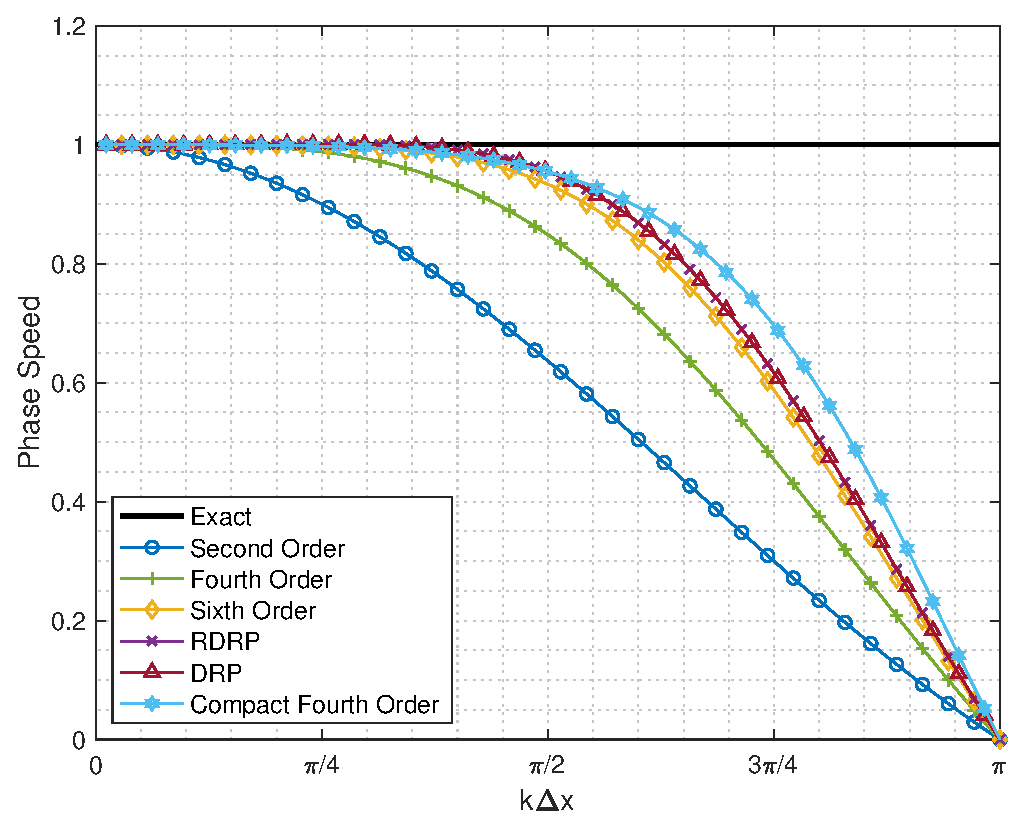
\includegraphics[width=0.6\textwidth]{Figures/Phase_Speed}}
	\caption{Convection Speed Comparison}
	\label{fig:alpha}
\end{figure}

\noindent
The maximum order of accuracy first derivative schemes are:
\begin{equation*}
	\begin{split}
		\left.\frac{\partial{u}}{\partial{x}}\right|_{i}~=&~\frac{u_{i+1}-u_{i-1}}{2\Delta{x}} +\varphi\left(\Delta{x^2}\right) \\
		\left.\frac{\partial{u}}{\partial{x}}\right|_{i}~=&~\frac{-u_{i+2}+8u_{i+1}-8u_{i-1}+u_{i-2}}{12\Delta{x}}  +\varphi\left(\Delta{x^4}\right) \\
		\left.\frac{\partial{u}}{\partial{x}}\right|_{i}~=&~\frac{u_{i+3}-9u_{i+2}+45u_{i+1}-45u_{i-1}+9u_{i-2}-u_{i-3}}{60\Delta{x}}  +\varphi\left(\Delta{x^6}\right) 
	\end{split}
\end{equation*}
Tam and Shen DRP \cite{DRP} and Hixon RDRP \cite{RDRP} schemes are widely robust optimized schemes given as:
\begin{itemize}
	\item DRP:
		\begin{equation*}
			\left.\frac{\partial{u}}{\partial{x}}\right|_{i}~=~\frac{1}{\Delta{x}}
				\left(\begin{matrix} 	
					~~0.0208431427703u_{i+3} 
					-~0.166705904415u_{i+2}  
					+~00.570882380518u_{i+1}  \\
					-~00.570882380518u_{i-1}  
					+~0.166705904415u_{i-2}  
					-~0.0208431427703u_{i-3}
				\end{matrix}
				\right)+\varphi\left(\Delta{x^4}\right) 
		\end{equation*}
	\item RDRP:
		\begin{equation*}
			\left.\frac{\partial{u}}{\partial{x}}\right|_{i}~=~\frac{u_{i+3}-8u_{i+2}+37u_{i+1}-37u_{i-1}+8u_{i-2}-u_{i-3}}{48\Delta{x}}+\varphi\left(\Delta{x^4}\right) 
		\end{equation*}
\end{itemize}
However, an issue when using large stencil sizes for implicit schemes is that the matrix on the LHS is expensive to solve (due to the number of diagonals). 

In order to decrease the computational work faced when solving for the flow variable $\{\Delta{Q}_i\}$, the LHS matrix is approximated (preconditioned) using second-order differences while maintaining high-order differences in the physics of the governing equations. For example, solving the governing equations using the RDRP differencing stencil:
\begin{equation}
	\label{eq:RDRP_NS}
  		\left[I+\Delta{t}\left(\frac{A_{i+3}-8A_{i+2}+37A_{i+1}-37A_{i-1}+8A_{i-2}-A_{i-3}}{48\Delta{x}}\right)^{n+1,l}\right]\Delta{Q}_i~=~-\Delta{t}\left\{RHS\right\}_i^{n+1, l}
\end{equation}
is preconditioned as:
\begin{equation}
	\label{eq:TriDi_NS}
  		\left[I+\Delta{t}\left(\frac{A_{i+1}-A_{i-1}}{2\Delta{x}}\right)^{n+1,l}\right]\Delta{Q}_i~=~-\Delta{t}\left\{RHS\right\}_i^{n+1, l}
\end{equation}
where $\left\{RHS\right\}_i^{n+1, l}$ in Eq. (\ref{eq:RDRP_NS}) \textbf{and} Eq. (\ref{eq:TriDi_NS}) is: 
\begin{equation*}
	\left\{RHS\right\}_i^{n+1, l}~=~\left(\frac{Q_i^{n+1, l}-Q_i^n}{\Delta{t}}+\frac{\partial}{\partial{x}}\left(\frac{E_{i+3}-8E_{i+2}+37E_{i+1}-37E_{i-1}+8E_{i-2}-E_{i-3}}{48\Delta{x}}\right)^{n+1,l}\right)
\end{equation*}
Approximation made to the LHS matrix will cause numerical errors, which can yield instability. A von Neumann stability analysis is performed to check the stability of the preconditioned implicit time step. 

\section{Stability for a Preconditioned Implicit Scheme}
\label{sec:Stability}
\subsection{Fourier or Von Neumann Analysis}
The Fourier or Von Neumann stability analysis checks the stability of finite difference schemes once applied to PDEs. The truncation error for the inviscid convection equation is defined as:
\begin{equation*}
	u_i^n~=~D_i^n+\epsilon_i^n
\end{equation*}
where $D$ exactly satisfies the discretized equation. Substituting in and eliminating $D$ gives the error equation:
\begin{equation}
	\begin{split}
		\label{eq:Implicit_Scheme_Error}
  			\frac{\partial{\epsilon}}{\partial{t}} +\left(c\cdot\frac{\partial{\epsilon}}{\partial{x}}\right)^{n+1}~=~0
	\end{split}
\end{equation}
Assuming that the error is a linear combination of Fourier modes in space: 
\begin{align}
		\label{eq:Error_Fourier}
  			\epsilon^n~=&~\sum_{k=-\frac{\pi}{\Delta{x}}}^{\frac{\pi}{\Delta{x}}}{A_k^n e^{jkx}} & 
  			\epsilon^{n+1}~=&~\sum_{k=-\frac{\pi}{\Delta{x}}}^{\frac{\pi}{\Delta{x}}}{A_k^{n+1} e^{jkx}} &
  			\Delta{\epsilon}~=&~\sum_{k=-\frac{\pi}{\Delta{x}}}^{\frac{\pi}{\Delta{x}}}{\Delta{A_k} e^{jkx}} 
\end{align}
substituting into equation (\ref{eq:TriDi_NS}), and defining:
\begin{equation*}
	\nu~=~\frac{c\Delta{t}}{\Delta{x}}
\end{equation*}
gives the equation for each Fourier mode as:
\begin{equation}
	\begin{split}
		\label{eq:Fourier_Mode_LHS_neq_RHS}
   			\Delta{\epsilon}+\frac{\nu}{2}\left(\Delta{\epsilon_{i+1}}-\Delta{\epsilon_{i-1}} \right)~=&~-\Delta{t}\left(\left.\frac{\partial}{\partial{x}}\right|_{RHS}\left( c \right)\right) {\epsilon}_i^{n} \\
  			\left|\frac{A_k^{n+1}}{A_k^{n}} \right|^2~=&~1+\frac{\nu^2\alpha_2\left(\alpha_2-2\alpha_1\right)}{1+\nu^2\alpha_1^2}
	\end{split}
\end{equation}
where $\alpha_1$ and $\alpha_2$ are the second order and RHS difference errors in the numerical convection speed, respectively. 
A finite difference scheme is stable if the errors made at one-time step of the calculation do not cause the errors to be amplified. 
Such a scheme exists if the amplification factor is less than or equal to one. 

It can be proved stability is only possible in Eq. (\ref{eq:Fourier_Mode_LHS_neq_RHS}) at high CFL if:
\begin{equation*}
	\alpha_2-2\alpha_1 \leq 0
\end{equation*}
Plotting the phase speed error difference (Fig. \ref{fig:alpha_stability}), instability is present at high wavenumbers. If Eq. (\ref{eq:Fourier_Mode_LHS_neq_RHS}) is approximated once again such that a scaling factor is multiplying the second order difference:
\begin{equation}
	\begin{split}
		\label{eq:Fourier_Mode_LHS_neq_RHS_Scaling}
   			\Delta{\epsilon}+\frac{\sigma\nu}{2}\left(\Delta{\epsilon_{i+1}}-\Delta{\epsilon_{i-1}} \right)~=&~-\Delta{t}\left(\left.\frac{\partial}{\partial{x}}\right|_{RHS}\left( c \right)\right) {\epsilon}_i^{n} \\
  			\left|\frac{A_k^{n+1}}{A_k^{n}} \right|^2~=&~1+\frac{\nu^2\alpha_2\left(\alpha_2-2\sigma\alpha_1\right)}{1+\nu^2\sigma^2\alpha_1^2}
	\end{split}
\end{equation}
for stability:
\begin{equation*}
	\alpha_2-2\alpha_1\sigma \leq 0
\end{equation*}
and the scaling factor values are shown in Table \ref{tab:Scaling}. Hence the scaling factor is physically insuring the numerical errors from the second-order difference can overcome the numerical errors from the RHS differencing stencil. Finally, the new preconditioned scheme can be written as follows: 
\begin{equation}
	\label{eq:TriDi_NS_Scaling}
  		\left[I+\Delta{t}\sigma\left(\frac{A_{i+1}-A_{i-1}}{2\Delta{x}}\right)^{n+1,l}\right]\Delta{Q}_i~=~-\Delta{t}\left\{RHS\right\}_i^{n+1, l}
\end{equation}
this will be referred to as tridiagonal matrices with scaling factors. 


\begin{figure}[hbt!]
	\centering
	{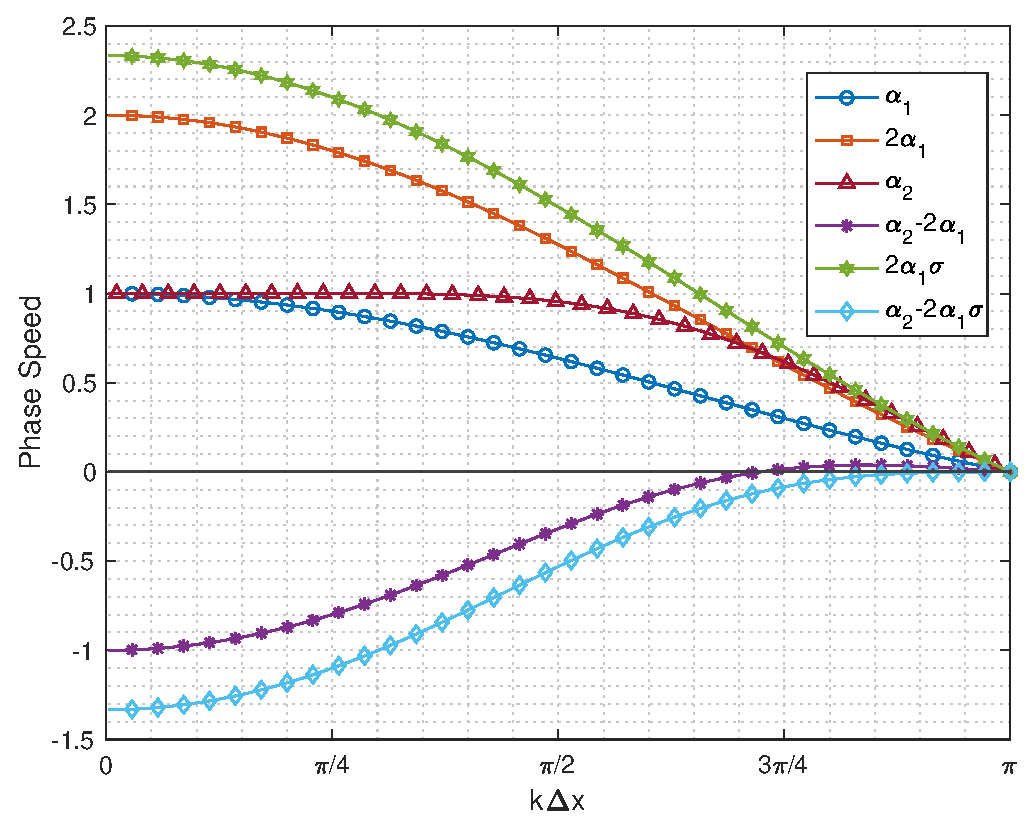
\includegraphics[width=0.6\textwidth]{Figures/Phase_2alpha_sigma}}
	\caption{Convection Speed, $\alpha_1=\left(\frac{\left(k\Delta{x}\right)^*}{k\Delta{x}} \right)_{E2}$ and $\alpha_2=\left(\frac{\left(k\Delta{x}\right)^*}{k\Delta{x}} \right)_{RDRP}$}
	\label{fig:alpha_stability}
\end{figure}

\subsection{Bounded Flow and Scaling Factors}
\label{subsec:Bounded_Scaling}
%Before examining the benchmark problems and validating the periodic scaling factor values obtained, it is essential to compute the scaling factors with bounded flow.
For problems with periodic boundary conditions, the Fourier analysis presented above may be used to assess the global errors and calculate periodic scaling factors. 
However, this is not possible with other boundary conditions, such as a bounded flow. 
Hence an eigendecomposition is needed to calculate the numerical stability of a time step. 
For this analysis, the Hixon et al. 'ghost point correction' method is used, \cite{GPT, RDRP} in which the governing equations are directly solved at the boundary points. 
Values of the bounded scaling factors are calculated numerically and shown in Table \ref{tab:Scaling}


%Consider a one-dimensional linear advection case discretized into $N$ equal intervals in space. 
%A second-order spatial difference is used on the LHS, and the governing equation is:
%\begin{equation}
%	\begin{split}
%		\label{eq:LAE}
%  			\left(I+\Delta{t}\cdot\left(\left.\frac{\partial}{\partial{x}}\right|_{LHS}\left(c\right)\right)\right)\Delta{u}~=&~-\Delta{t}\left(\left.\frac{\partial}{\partial{x}}\right|_{RHS}\left(c\right)\right) {u}_i^{n} \\
%  			\Delta{u}+\frac{\sigma\nu}{2}\left(\Delta{u_{i+1}}-\Delta{u_{i-1}} \right)~=&~-\Delta{t}\left(\left.\frac{\partial}{\partial{x}}\right|_{RHS}\left(c\right)\right) {u}_i^{n} \\
%  			\left[A\right]\left\{\Delta{u}\right\}~=&~\left[B\right]\left\{u_{i}^{n}\right\} \\
%	\end{split}
%\end{equation}
%Where $[A]$ and $[B]$ are $N\times{N}$ (sparse) matrices and $\Delta{u},~u_{i}^{n}$ are $N$ vectors representing the value of the function at the nodes $x_i~=~i/N$.
%To analyze the stability of a time step, re-write Eq. (\ref{eq:LAE}) as:
%\begin{equation}
%\label{eq:AB}
%	\begin{split}
%  		[A]\{\Delta{u_i\}}~=&~[B]\{u_i^{n}\} \\
%  		\left\{\frac{\Delta{u_i}}{u_i^{n}}\right\}~=&~[A]^{-1}[B] \\
%  		\frac{u_i^{n+1}}{u_i^{n}} - [1]~=&~[A]^{-1}[B] \\
%  		\frac{u_i^{n+1}}{u_i^{n}}~=&~[A]^{-1}[B] + [1] \\
%  		~=&~[C]
%	\end{split}
%\end{equation}
%The eigenvalues are calculated as follows:
%\begin{equation}
%	\begin{split}
%		\label{eq:Magnitude_Of_Eigen}
%  			\left|\frac{u_i^{n+1}}{u_i^{n}}\right|~=~\left|\lambda\left[C\right]\right|
%	\end{split}
%\end{equation}
%If the magnitude of the eigenvalues is less than or equal to one, then the time step is stable.  
%Otherwise, error terms will amplify, and the time step will be unstable.
%Note that matrices $[A]$ and $[B]$ are functions of the CFL, $\nu$. 
%Therefore the eigenvalues obtained are also functions of $\nu$. 
%
%For this analysis, all schemes use the Hixon et al. 'ghost point correction' method, \cite{GPT, RDRP} in which the governing equations are directly solved at the boundary points. 
%As described in the reference, the spatial derivatives are first computed for all directions, using the '\textit{noBC}' stencils in the direction normal to the boundary. 
%The boundary conditions of:
%\begin{equation}
%	\begin{split}
%		\label{eq:}
%  			\left.\frac{\partial{u}}{\partial{x}}\right|_i^{BC}~=~0
%	\end{split}
%\end{equation}
%is then applied as a 'correction' to the normal derivative at the boundary, modifying the flux value at a nonphysical' ghost point' outside the computational domain.
%This modified ghost point value affects the normal derivative at every grid point whose spatial derivative uses the ghost point value. 
%These corrections are given in terms of the boundary normal derivative correction on the appropriate grid line in the reference \cite{GPT, RDRP}. 

%\subsection{LU-SGS Stability}
%\label{subsec:LUSGS}
%Yoon and Jameson's LU-SGS numerical time-step stability is analyzed in this section. The eigendecomposition setup explained in Section \ref{subsec:Bounded_Scaling} is used again here.
%Consider a periodic one-dimensional linear advection case that is discretized into $N$ equal intervals in space; the LU-SGS method is written as:
%\begin{equation}
%	\begin{split}
%	\label{eq:LSGSU_LAE}
%		LD^{-1}U\Delta{u}~=&~-\Delta{t}\left\{RHS\right\}^{n}_i
%	\end{split}
%\end{equation}
%note that using the linear advection equation, the jacobian of the flux, $A$, and the corresponding eigenvalue are:
%\begin{equation}
%	\begin{split}
%		\label{eq:FluxJac_Eig}
%  			A~=&~\frac{\partial{E}}{\partial{Q}}~=~c \\
%  			\epsilon_A~=&~c
%	\end{split}
%\end{equation}
%giving the decomposed positive and negative eigenvalues, $A^+$ and $A^-$ respectively:
%\begin{equation}
%	\begin{split}
%		\label{eq:A_Plus_Minus}
%  			A^{+}~=&~\frac{1}{2}\left(A+\epsilon_AI\right)~=~c \\
%  			A^{-}~=&~\frac{1}{2}\left(A-\epsilon_AI\right)~=~0
%	\end{split}
%\end{equation}
%thus:
%\begin{equation}
%	\label{eq:LDU}
%	\begin{split}
%            L~=&~I + \alpha\Delta{t}\left(D_x^-A^+\right)\\
%		D~=&~I + \alpha\Delta{t}\left(A^+\right) \\
%		U~=&~I + \alpha\Delta{t}\left(A^+\right)
%	\end{split}
%\end{equation}
%where $D_x^-$ is a \textit{first order backward difference operator}.  
%To analyze the stability of a time step, re-write Eq. (\ref{eq:LSGSU_LAE}) as:
%\begin{equation}
%\label{eq:AB}
%	\begin{split}
%  		[L][D]^{-1}[U]\{\Delta{u_i\}}~=&~[B]\{u_i^{n}\} \\
%  		[A]\{\Delta{u_i\}}~=&~[B]\{u_i^{n}\} \\
%  		\frac{u_i^{n+1}}{u_i^{n}}~=&~[A]^{-1}[B] + [1] \\
%  		~=&~[C]
%	\end{split}
%\end{equation}
%The eigenvalues are calculated as:
%\begin{equation}
%	\begin{split}
%		\label{eq:Magnitude_Of_Eigen}
%  			\left|\frac{u_i^{n+1}}{u_i^{n}}\right|~=~\left|\lambda\left[C\right]\right|
%	\end{split}
%\end{equation}
%If the magnitude of the eigenvalues is less than or equal to one, then the time-step is stable.   
%The most striking result to emerge from the data is with periodic and bounded flow, no scaling factors are needed when using the LU-SGS factorization on the LHS as seen in Table (\ref{tab:Scaling}). 

\begin{table}[htp!]
\centering
\caption{Periodic and Bounded Flow Scaling Factors}
\begin{tabular}{|l|c|c|c|c|c|c|}
\hline
 & \multicolumn{1}{c|}{\textbf{$\sigma_{E2}$}} & \multicolumn{1}{c|}{\textbf{$\sigma_{E4}$}} & \multicolumn{1}{c|}{$\sigma_{E6}$} & \multicolumn{1}{c|}{$\sigma_{DRP}$} & \multicolumn{1}{c|}{$\sigma_{RDRP}$}& \multicolumn{1}{c|}{$\sigma_{C4}$}\\ \hline
\textbf{Periodic} & \textit{1.0} & \textit{1.0} & \textit{$\nicefrac{11}{10}$} & \textit{1.166823} & \textit{$\nicefrac{7}{6}$} & \textit{1.49982}\\ \hline
%\textbf{LUSGS-Periodic} & \textit{1.0} & \textit{1.0} & \textit{1.0} & \textit{1.0} & \textit{1.0} & \textit{1.0}\\ \hline
\textbf{Bounded} & \textit{1.0} & \textit{2.12179} & \textit{6.3527} & 
	\textit{4.97487} & 
	\textit{6.36206}& 
	\textit{3.80018}\\ \hline
%\textbf{LUSGS-Bounded} & \textit{1.0} & \textit{1.0} & \textit{1.0} & \textit{1.0} & \textit{1.0} & \textit{1.0}\\ \hline
\end{tabular}
\label{tab:Scaling}
\end{table}
\pagebreak
\section{Numerical Results for Benchmark
Problems}
%One way to analyze the stability of an implicit time step was shown in Section \ref{sec:Stability}; 
%form the associated matrices using a finite number of points. Then use computer software to compute the eigenvalues, which can then be used to quantify the stability nature of each scheme. 
%While this does provide at least a first-order measure of linear stability, the analysis is by no means rigorous or general. 
%Hence, real-life nonlinear benchmark steady problems are studied in this section to validate the conclusions from the eigenvalue analysis. 

In Computational Fluid Dynamics and Computational Aeroacoustics, emphasis is given to calculating both the steady and unsteady flow. 
Various numerical schemes are developed to correctly understand and predict noise generation and propagation physics. 
To verify the correct implementation of those schemes and their performances, a range of validation problems with solutions are listed in the CAA Workshops \cite{CAA1, CAA2, CAA3}.

This paper studies one problem from the Third CAA workshop: \textit{Category 1 Problem 1} \cite{CAA3}. 
Category 1 problems deal with internal propagation; 
the propagation of sound through a narrow passage with flow exists in many applications. 
Problem 1 models the upstream propagation of sound through a nozzle with near sonic conditions. 
The Quasi-1D nonlinear Euler equations are used to solve this problem:
\begin{equation}
    \label{eq:Euler}
    \frac{\partial{}}{\partial{t}} 
    \begin{Bmatrix}
        \rho \\
        \rho{u} \\
        E_{tot}
  \end{Bmatrix}+\frac{\partial{}}{\partial{x}}
    \begin{Bmatrix}
        \rho{u} \\
        \rho{u^2}+p \\
        u(E_{tot}+p)
  \end{Bmatrix} +\frac{1}{A}\frac{\partial{A}}{\partial{x}}
    \begin{Bmatrix}
        \rho{u} \\
        \rho{u^2} \\
        u(E_{tot}+p)
  \end{Bmatrix}= 0
\end{equation}
For the time step, the CFL parameter $\nu$ is defined as:
\begin{equation}
	\begin{split}
		\label{eq:}
  			\nu_{physical}
  			~=&~\frac{\left(\left|u_i\right|+c_i\right)\Delta{t}}{\Delta{x}}\cdot\left(k\Delta{x}\right)^*
	\end{split}
\end{equation}
The area of the duct is given by:
\begin{equation}
	\begin{split}
		\label{eq:}
  			A(x)~=&~\left\{
  			\begin{matrix}
  				0.536572~-~0.198086e^{\left(-ln2\right)\left(\frac{x}{0.6}\right)^2} & x \geq 0 \\
  				1.0~-~0.661514e^{\left(-ln2\right)\left(\frac{x}{0.6}\right)^2} & x \leq 0
  			\end{matrix}
  			\right.
	\end{split}
\end{equation}
on a computational domain of $-10\leq~x~\leq10$. 
%The duct area vs. domain is shown in Fig. \ref{fig:Domain_Area}.



%The mean stagnation pressure and density are calculated as:
%\begin{equation}
%    \label{eq:Euler_BC_2}
%    \begin{split}
%    \overline{p_0}~= & ~\overline{p}\left(1+\frac{\gamma -1}{2}\overline{M}^2\right)^{\frac{\gamma}{\gamma-1}} \\
%    \overline{\rho_0}~= & ~\overline{\rho}\left(1+\frac{\gamma -1}{2}\overline{M}^2\right)^{\frac{1}{\gamma-1}} \\
%    \overline{M} ~ = & ~ \frac{\overline{u}}{\overline{c}} \\
%    \overline{c} ~ = & ~ \sqrt{\frac{\gamma{\overline{p}}}{\overline{\rho}}}
%    \end{split}
%\end{equation}
%mean flow conditions such as $\left(\overline{\rho},~\overline{u},~\overline{p} \right)$ are specified for each problem. 
%

The numerical solver for this work uses an implicit time marching scheme with
the preconditioned matrix on LHS. 
The LHS spatial difference is coupled with scaling factors for stability. 
While the following spatial differences are used on the RHS:
\begin{itemize}
	\item Second Order (E2)
	\item Fourth Order (E4)
	\item Sixth Order (E6)
	\item DRP  (DRP)
	\item RDRP  (RDRP)
	\item Prefactored Fourth Order Compact (C4)
\end{itemize}
In order to accurately predict the flow, it is crucial to apply the boundary conditions correctly; otherwise, the boundaries may (and will) generate spurious fluctuations and thereby contaminate the entire solution. 
Thompson's nonlinear boundary conditions are used in this paper (referred to as characteristic boundaries in the literature) \cite{Thompson1, Thompson2}.  
%The Thompson approach \cite{Thompson1, Thompson2} uses an eigendecomposition on the Euler flux Jacobian matrix to generate the eigenvalues and eigenvector matrices, which are then used to diagonalize and decompose the equations. 
%This decomposition generates three equations, when compared to the linear advection equation, can classify three different waves:
%\begin{enumerate}
%	\item An entropy wave, convecting with the flow:
%		\begin{equation*}
%			\frac{\partial{A_s}}{\partial{t}}~=~p_t-c^2\rho_t
%		\end{equation*}
%	\item A downstream-running acoustic wave, convecting with the flow and propagating downstream at the speed of sound:
%		\begin{equation*}
%			\frac{\partial{A_+}}{\partial{t}}~=~p_t+\rho{c}u_t
%		\end{equation*}
%	\item An upstream-running acoustic wave, convecting with the flow and propagating upstream at the speed of sound:
%		\begin{equation*}
%			\frac{\partial{A_-}}{\partial{t}}~=~p_t-\rho{c}u_t
%		\end{equation*}
%\end{enumerate}
%Following Thompson's approach, waves leaving the domain are left unspecified. 
%The calculations of such waves are determined using a one-sided difference. 
%Waves that are entering the domain must be specified.

%For both Category 1 problems, the inflow and outflow boundaries are subsonic. 
%An entropy and downstream running acoustic waves are specified using the mean stagnation pressure and mean stagnation density for the inflow boundary.
%The outflow boundary specifies the upstream-running acoustic wave using the mean exit pressure. 

%\begin{figure}[hbtp!]
%	\centering
%{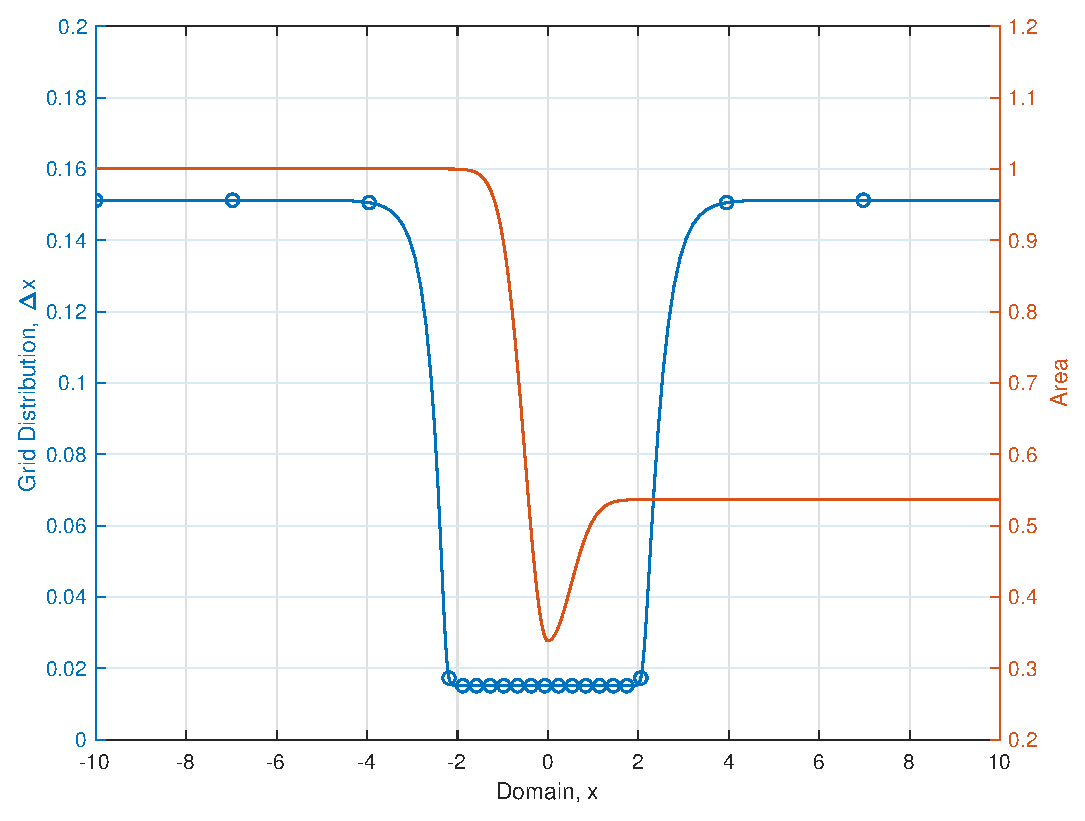
\includegraphics[width=00.5\textwidth]{Figures/Area_dX}}
%  	\caption{Category 1 Problem 1 Domain vs. Area and Grid Distribution}
%  	\label{fig:Domain_Area}
%\end{figure}
 
\subsection{Category 1 Problem 1: Propagation of Sound Waves through a Transonic Nozzle}

The problem is the upstream propagation of an acoustic wave through a transonic, nearly choked nozzle flow. 
The mean flow is set as follows:
\begin{equation*}
	\left\{
	\begin{matrix}
		\overline{\rho} \\
		\overline{u} \\
		\overline{p}
	\end{matrix}
	\right\}~=~
	\left\{
	\begin{matrix}
		1.0 \\
		0.4 \\
		\frac{1}{\gamma}
	\end{matrix}
	\right\}
\end{equation*}
An explicit tenth-order Kennedy and Carpenter's artificial dissipation operator that provides damping for the inviscid nonlinear calculations is added to the equation \cite{Kennedy_Carp}. The initial condition is set to the mean flow values to solve the steady mean distribution. 

In this test case, an inviscid flow travels through a converging-diverging nozzle. 
This is a fully subsonic flow since there is no discontinuity in pressure.
A pressure drop is expected as the flow accelerates through the throat and then rises again as the flow backs down in Fig. \ref{fig:C1P1_SteadyState}.  
The convergence of each scheme was determined by calculating the residual of the fluxes. 
Figure \ref{fig:C1P1_ROC} shows the residual vs. iteration for the schemes. 
The Figure indicates converged solutions for the various RHS difference formulation. 
A value of $\Delta{t}\to\infty$ is set such that the LHS schemes reduce to a Newton iteration. 
%However, the unsteady results are calculated to highlight the effect of higher-order difference stencils.  

Once the steady mean-flow results are obtained, the upstream propagating perturbation starts at the boundary, and the unsteady results are studied.  
Here, a small amplitude acoustic wave is generated way downstream and propagates upstream through the narrow passage of the nozzle throat:
\begin{equation*}
	\left\{
	\begin{matrix}
		{\rho}' \\
		{u}' \\
		{p}'
	\end{matrix}
	\right\}_{outflow}~=~
\epsilon
	\left\{
	\begin{matrix}
		1 \\
		-1 \\
		1
	\end{matrix}
	\right\}\cos\left[\omega\left(\frac{x_{outflow}}{1-M_{outflow}}+t\right)\right]
\end{equation*}
where $\epsilon=10^{-5}$ and $\omega=0.6\pi$. 

%The inflow boundaries are set to:
%\begin{equation*}
%	\begin{split}
%		\label{eq:}
%  			\left.\frac{\partial{A_s}}{\partial{t}}\right|_{inflow}~=&~0 \\
%  			\left.\frac{\partial{A_+}}{\partial{t}}\right|_{inflow}~=&~0
%	\end{split}
%\end{equation*}
%where the outflow is:
%\begin{equation*}
%	\left.\frac{\partial{A_-}}{\partial{t}}\right|_{outflow}~=~
%		-2\epsilon\omega\cdot{\sin}\left[\omega\left(\frac{10}{1-0.4} +t\right) \right]
%\end{equation*}
%
%Initially, the problem was run with a uniformly-spaced grid to determine the necessary spacing at $x=0$ (the nozzle throat). 
%This was obtained at 1351 equally-spaced points, or a $\Delta{x}$ of 0.0148. 
%The minimum spacing was set, and the grids were stretched to a maximum $\Delta{x}$ of 0.148 and were uniform to the boundary. 
%%The stretched grid solutions were then compared with the exact solution for accuracy. 
%Figure \ref{fig:Domain_Deltax} shows the grid spacing distribution as a function of x. 

Figure \ref{fig:Unsteady_C1P1_closeup} show the maximum pressure perturbation using vs. flow domain. 
The unsteady solution, taken once a periodic steady state is reached, uses 32 steps per cycle. An optimized $2^{nd}$ order optimized backward difference formulation \cite{HixonImplicit} is used to approximate the time derivative:
\begin{equation}
	\begin{split}
		\label{eq:2ndOrderdQdT}
  			\left.\frac{\partial{Q}}{\partial{t}}\right|_i~=&~\frac{10Q_i^{n+1, l}-15Q_i^n+6Q_i^{n-1}-Q_i^{n-2}}{6\Delta{t}}
	\end{split}
\end{equation}
The unsteady CFL is calculated as:
\begin{equation*}
	\nu_{physical}
  			~=~\frac{\left(\left|u_i\right|+c_i\right)}{\Delta{x}}\cdot\left(\frac{2\pi}{\omega}\cdot\frac{1}{\cdot \text{Steps~Per~Cycle}}\right)\cdot\left(k\Delta{x}\right)^*
\end{equation*}

For each implicit solve, the solution is converged down to machine precision. It is seen that second-order spatial difference cannot accurately predict the pressure perturbation where the higher-order schemes agree very well with the exact. 
The value of $\nu_{physical}$ for each test case is shown in Table \ref{tab:C1P1_CFL}.   


%\begin{figure}[hbtp!]
%	\centering
%	{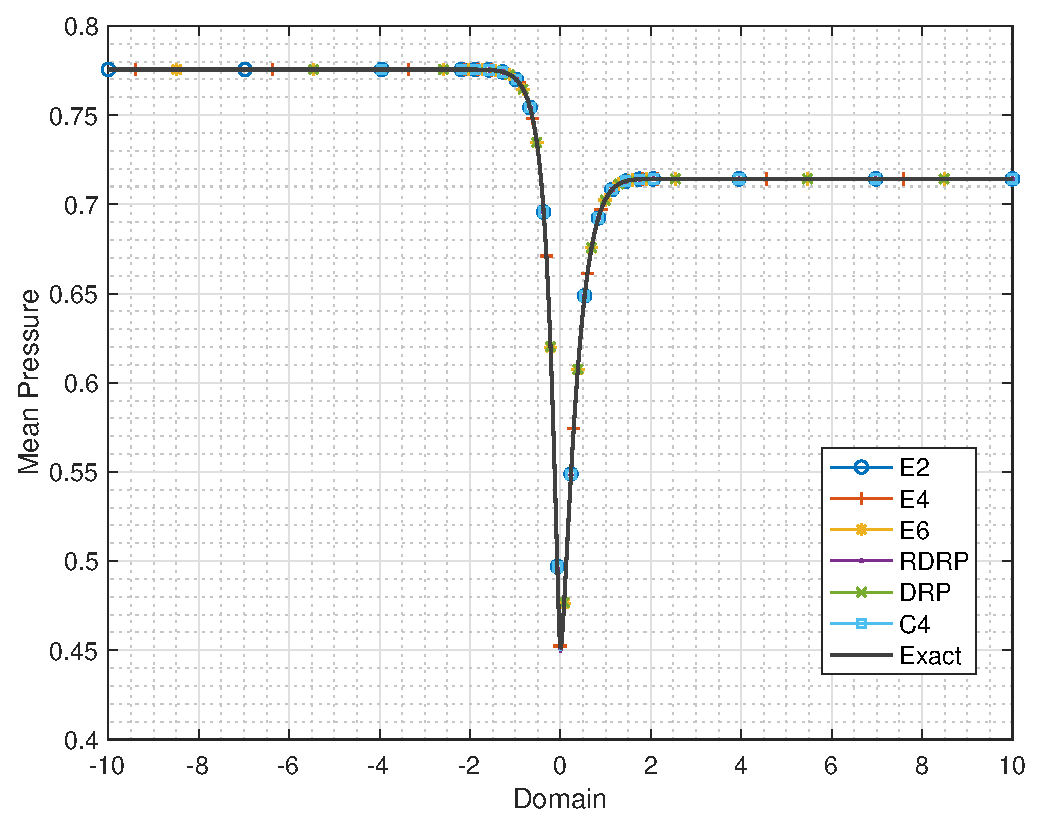
\includegraphics[width=0.5\textwidth]{Figures/C1P1_SteadyState}}
%	\caption{Domain vs Mean Pressure for Category 1 Problem 1}
%	\label{fig:C1P1_SteadyState}
%\end{figure}
%
%
%\begin{figure}[hbtp!]
%	\centering
%	{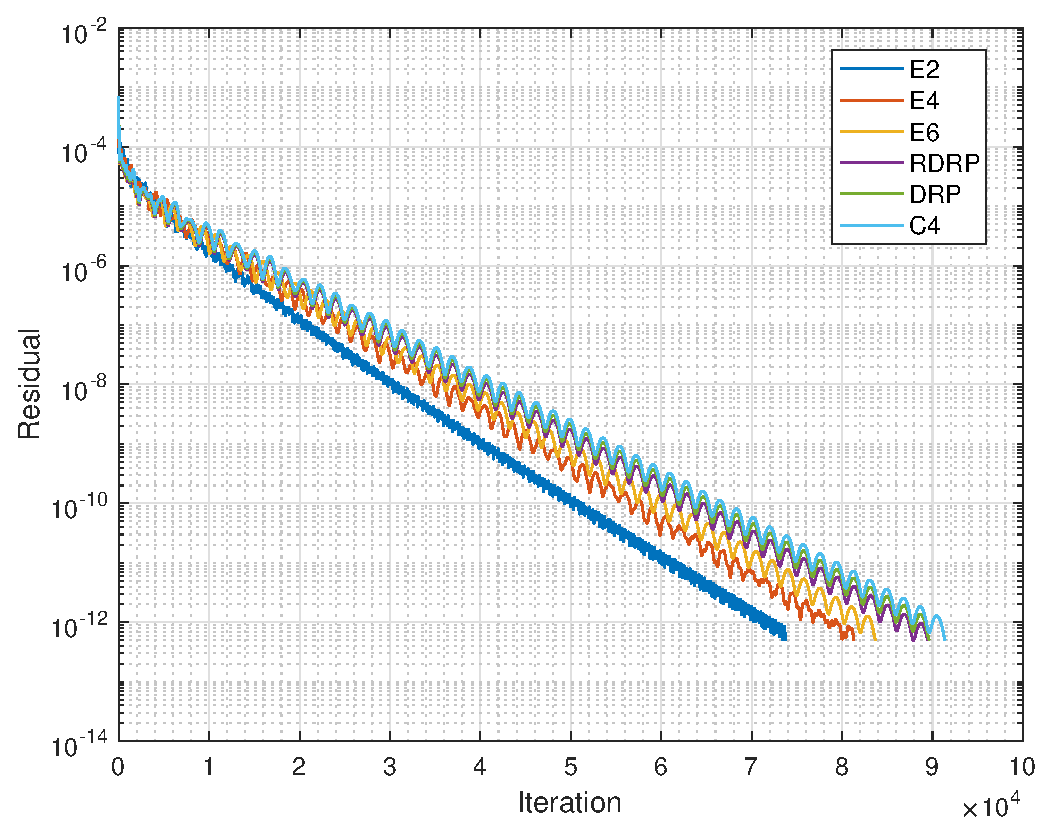
\includegraphics[width=0.5\textwidth]{Figures/C1P1_TriDi_Scaling_ROC}}
%	\caption{Residual vs Iteration Category 1 Problem 1}
%	\label{fig:C1P1_ROC}
%\end{figure}

\begin{figure}
\centering
\begin{minipage}{.5\textwidth}
  \centering
  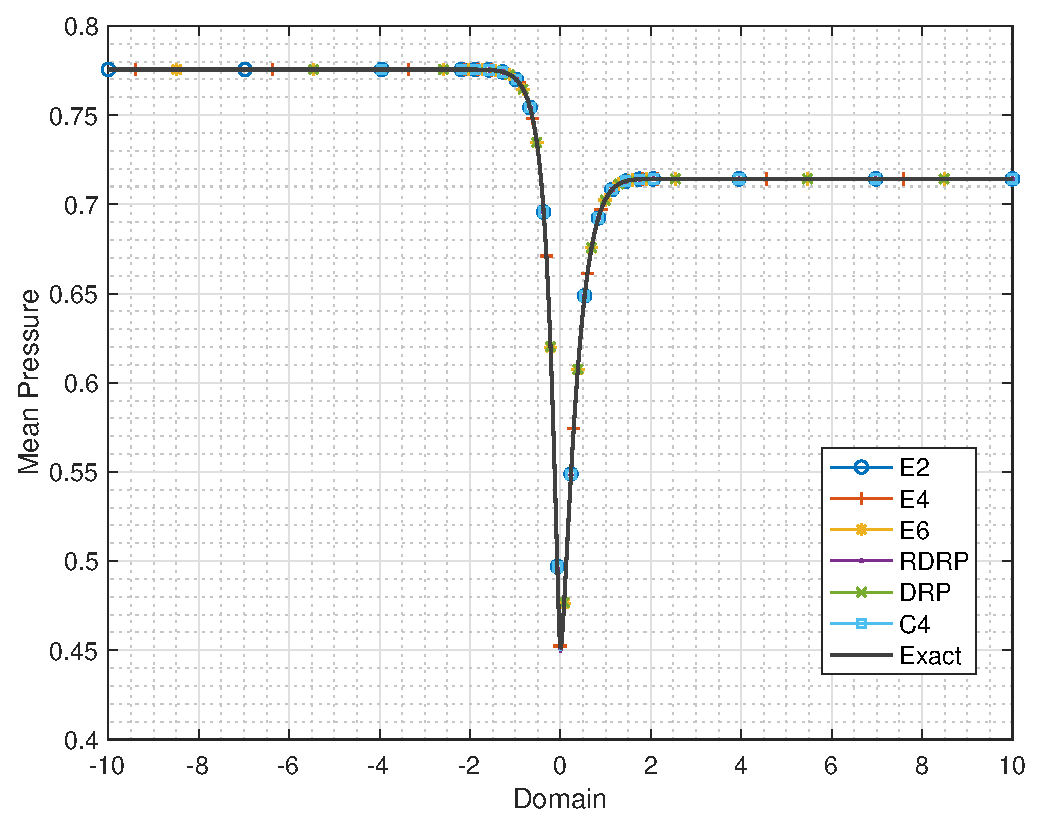
\includegraphics[width=0.95\linewidth]{Figures/C1P1_SteadyState}
  \captionof{figure}{Domain vs Mean Pressure}
  \label{fig:C1P1_SteadyState}
\end{minipage}%
\begin{minipage}{.5\textwidth}
  \centering
  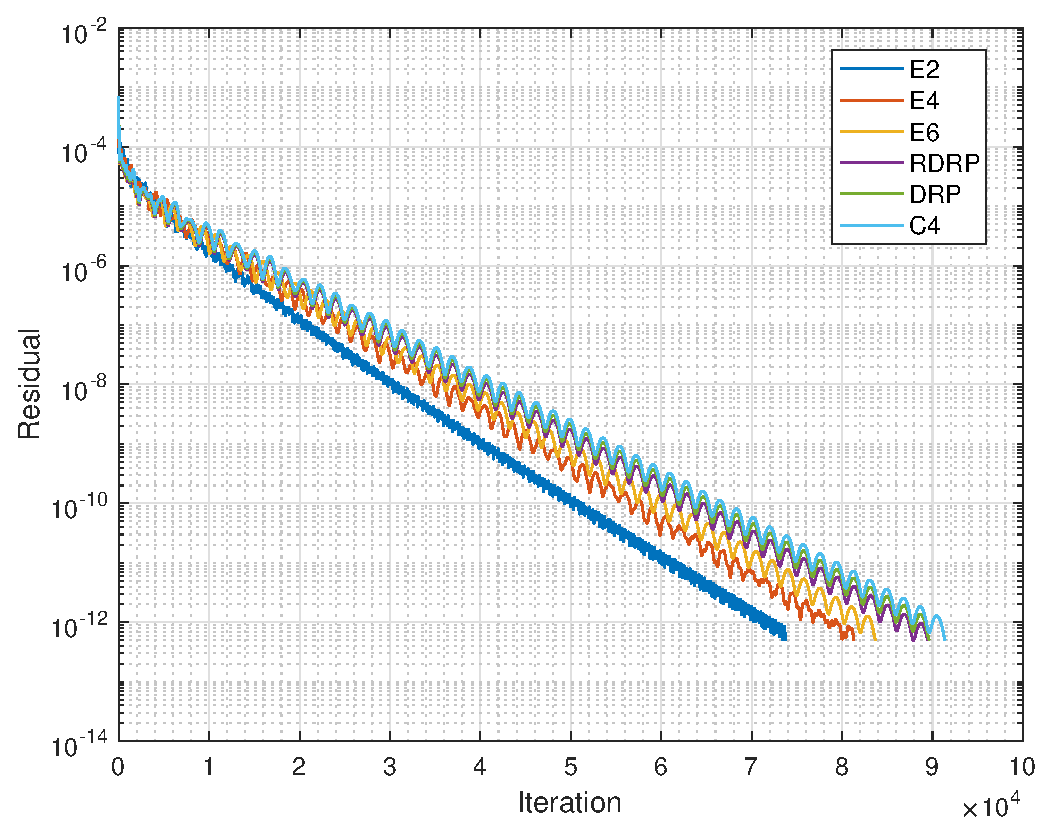
\includegraphics[width=0.95\linewidth]{Figures/C1P1_TriDi_Scaling_ROC}
  \captionof{figure}{Residual vs Iteration}
  \label{fig:C1P1_ROC}
\end{minipage}
\end{figure}

\begin{figure}[hbtp!]
	\centering
	{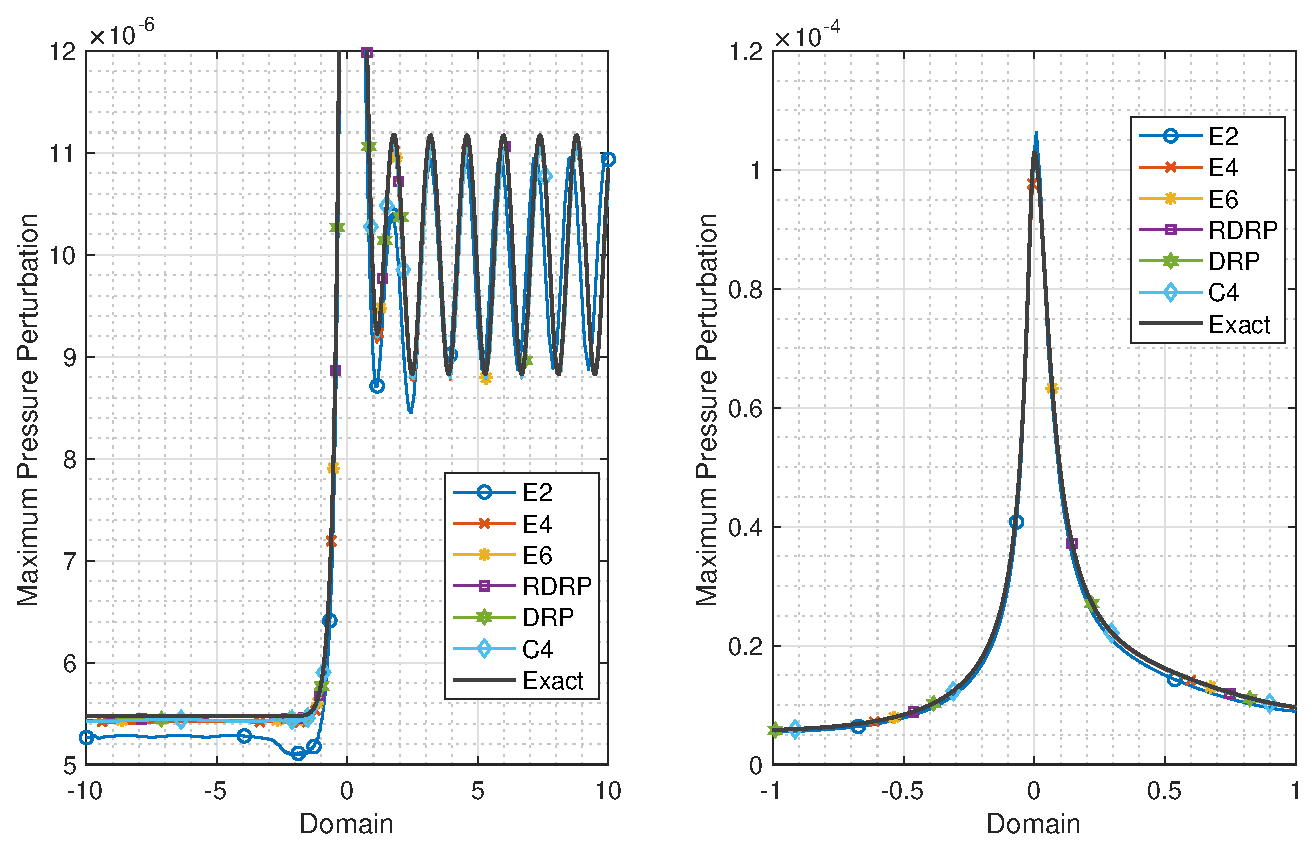
\includegraphics[width=1.0\textwidth]{Figures/C1P1_MaxDisturbance_zoom}}
	\caption{Maximum Pressure Disturbance for Category 1 Problem 1}
	\label{fig:Unsteady_C1P1_closeup}
\end{figure}

\begin{table}[htp!]
\centering
\caption{CFL Values for Category 1 Problem 1 from the CAA Workshop}
\label{tab:C1P1_CFL}
\begin{tabular}{|l|c|c|c|c|c|c|}
\hline
 & \multicolumn{1}{c|}{\textbf{E2}} & \multicolumn{1}{c|}{\textbf{E4}} & \multicolumn{1}{c|}{\textbf{E6}} & \multicolumn{1}{c|}{\textbf{DRP}} & \multicolumn{1}{c|}{\textbf{RDRP}}& \multicolumn{1}{c|}{\textbf{C4}}\\ \hline
\textbf{$\nu_{physical}$} & \textit{12.521} & \textit{17.518} & \textit{19.858} & \textit{20.834} & \textit{20.834} & \textit{22.237}\\ \hline
\end{tabular}
\end{table}


\section{Initial Conclusion and Proposed Work}
The present research aimed to establish a highly efficient implicit solver using higher-order spatial differencing schemes. 
Through the use of scaling factors, the LHS matrix was replaced with an easier-to-solve matrix hence cutting down on the computational work needed for the iterative steady-state solver. 
Although the current study is based on one-dimensional problems, the findings suggest stability is possible for traditional implicit formulation if scaling factors are used on the LHS spatial difference. 

For the final paper, the preconditioned matrix will be tested against Category 1 Problem 2 from the CAA workshop. The scheme's performance and convergence rate will be studied versus other indirect methods, such as the LU-SGS method, and adding implicit dissipation to stabilize the scheme. 

\section*{Acknowledgments}
This work was supported by the NASA Advanced Air Transportation Technologies (AATT) Project. The authors would like to thank Dr. Edmane Envia of the NASA Glenn Research Center, who was the technical monitor for this work.


\bibliography{sample}


\end{document}
